\documentclass[12pt]{article}
\RequirePackage{color,graphicx}
\graphicspath{ {images/} }
\usepackage{newcent}
\usepackage{multicol}
\usepackage{multirow}
\usepackage{cite}
\usepackage{url}
\usepackage{xltxtra,url,parskip}
\usepackage{xunicode}
\usepackage{float}
\usepackage[ruled,lined,linesnumbered,nofillcomment]{algorithm2e}
\usepackage[absolute]{textpos}
\usepackage[left=1.0in, right=1.0in, top=0.7in, bottom=0.7in]{geometry}
\usepackage[xetex,
  unicode,
  pdfencoding=auto,
  pdfinfo={
    Title={tjmaynes/Project3},
    Author={TJ Maynes},
    Subject={TJ Maynes Project3},
    Keywords={graphs, python, networkx, dijkstras, algorithms, undergraduate},
    Producer={xelatex},
    Creator{xelatex}}]{hyperref}
\defaultfontfeatures{Scale=MatchLowercase,Mapping=tex-text}
\defaultfontfeatures{Mapping=tex-text,Scale=MatchLowercase}
\restylefloat{table}

\begin{document}

\title{Graph Modeling Project}
\author{TJ Maynes}
\date{December 16, 2014}

\maketitle

\textbf{1 Problem Modeling}

 The problem is based on ``The Itsy Bitsy Spider'' maze problem from ``MAD MAZES: Intriguing Mind Twisters for Puzzle Buffs, Game Nuts and Other Smart People. This problem can be modeled as a undirected graph since we can represent the path taken to get from starting position to exit position as a series of nodes each connected by edges of neighboring nodes leading from source node to a desired node in a three dimensional graph. More specifically, we can represent each square on each level of the three dimensional maze as a node whose edge to a neighboring node is dependent on the direction that the node can take in the three dimensional graph. Also, if we represent the problem as a grpah, we can use a graphing algorithm to find all the different paths from source node(starting position) to the desired node(exit position). \\

\vspace{0.1in}
\textbf{1.1 Choose Your Data Structure}

We can use a dictionary data structure such as an adjacency list to represent each square on each level of the three dimensional maze as a node with node attributes that includes the directions we can take to a neighboring node. Each node can connect to a neighboring node based on the value of the node's attributes. Node attributes include: whether the color of square is floor (yellow sqaure) or a hole (white square), 1 indicates yellow and 0 indicates white; whether the node can travel north or not, 1 indicates there is a wall and 0 indicates we can travel to the next node; whether the node can travel south or not, 1 indicates there is a wall and 0 indicates we can travel to the next node; whether the node can travel east or node, 1 indicates there is a wall and 0 indicates we can travel to the next node; whether the node can travel west or not, 1 indicates there is a wall and 0 indicates we can travel to the next node. Also, each node will be represented by a unique value such as their position on the graph. For instance, the initial node would be represented as a position in the graph based on the level, row, column. Specifically from the maze problem, our initial node position would be (5,4,4) and our desired node position would be (1,1,1). This will allow us to uniquely identify the correct input values given to navigate the path from initial node to desired node in the three dimensional maze.\\

\vspace{0.1in}
\textbf{1.2 Creating the Graph}

Once we have created our data structure for our graph's nodes (and their node attributes) we can create a graph by connect each neighboring node based on their node attributes. In other words, we want to create an edge from node to node if that node can travel to that next node. For instance, our initial node (5,4,4) will look at it's nodes attributes to determine which direction that the node (at that current position) can go. In this instance, our initial node's attributes dictate that the node can only travel west to its neighboring node (5,4,3), so we create an edge between node (5,4,4) and neighboring node (5,4,3). We will continue creating an edge to each node by the current node's attributes until we have created last edge connecting our desired node. We can achieve this by creating a nested for-loop and a few if conditions which is described in Algorithm 1. \\

\begin{algorithm}
  \For{$k=1$ to $level+1$}{

    \For{$n=1$ to $width+1$}{

      \For{$m=1$ to $height+1$}{
        
        $addNode((k,n,m))$ with attributes

        \If{$node(k,n,m)[color] == 0$ and $k < level$}{
          addEdge((k,n,m),(k+1,n,m))
        }

        \If{$node(k,n,m)[south] == 0$ and $n < width$}{
          addEdge((k,n,m),(k,n+1,m))
        }

        \If{$node(k,n,m)[west] == 0$ and $m < height$}{
          addEdge((k,n,m),(k,n,m+1))
        }
      }
    }
  }
  \caption{\texttt{createGraph}($level, width, height$)}
\end{algorithm}

In Algorithm 1, you are allowed to start from k = 0 or k = 1, since the numbers are relative to the direction the node position will take to it's neighboring node. So long as you add the appropriate buffer to each loop (such as k = 1 to level + 1). I prefer to start from k = 1 since our desired node, in the case of the maze problem, is (1,1,1). Also, we create each if condition so that we can attach an edge based on what direction the node's, (k,n,m), attribute dictates. We do not need to check if the node is going north or east directions because that would cause the algorithm to add double edges between each neighboring node. Also, we only check if the node's attribute for color is going up since we are moving up through the maze. Also, if there is a floor you do not need to add an edge. \\

\vspace{0.1in}
\textbf{1.2 Graph Drawing}

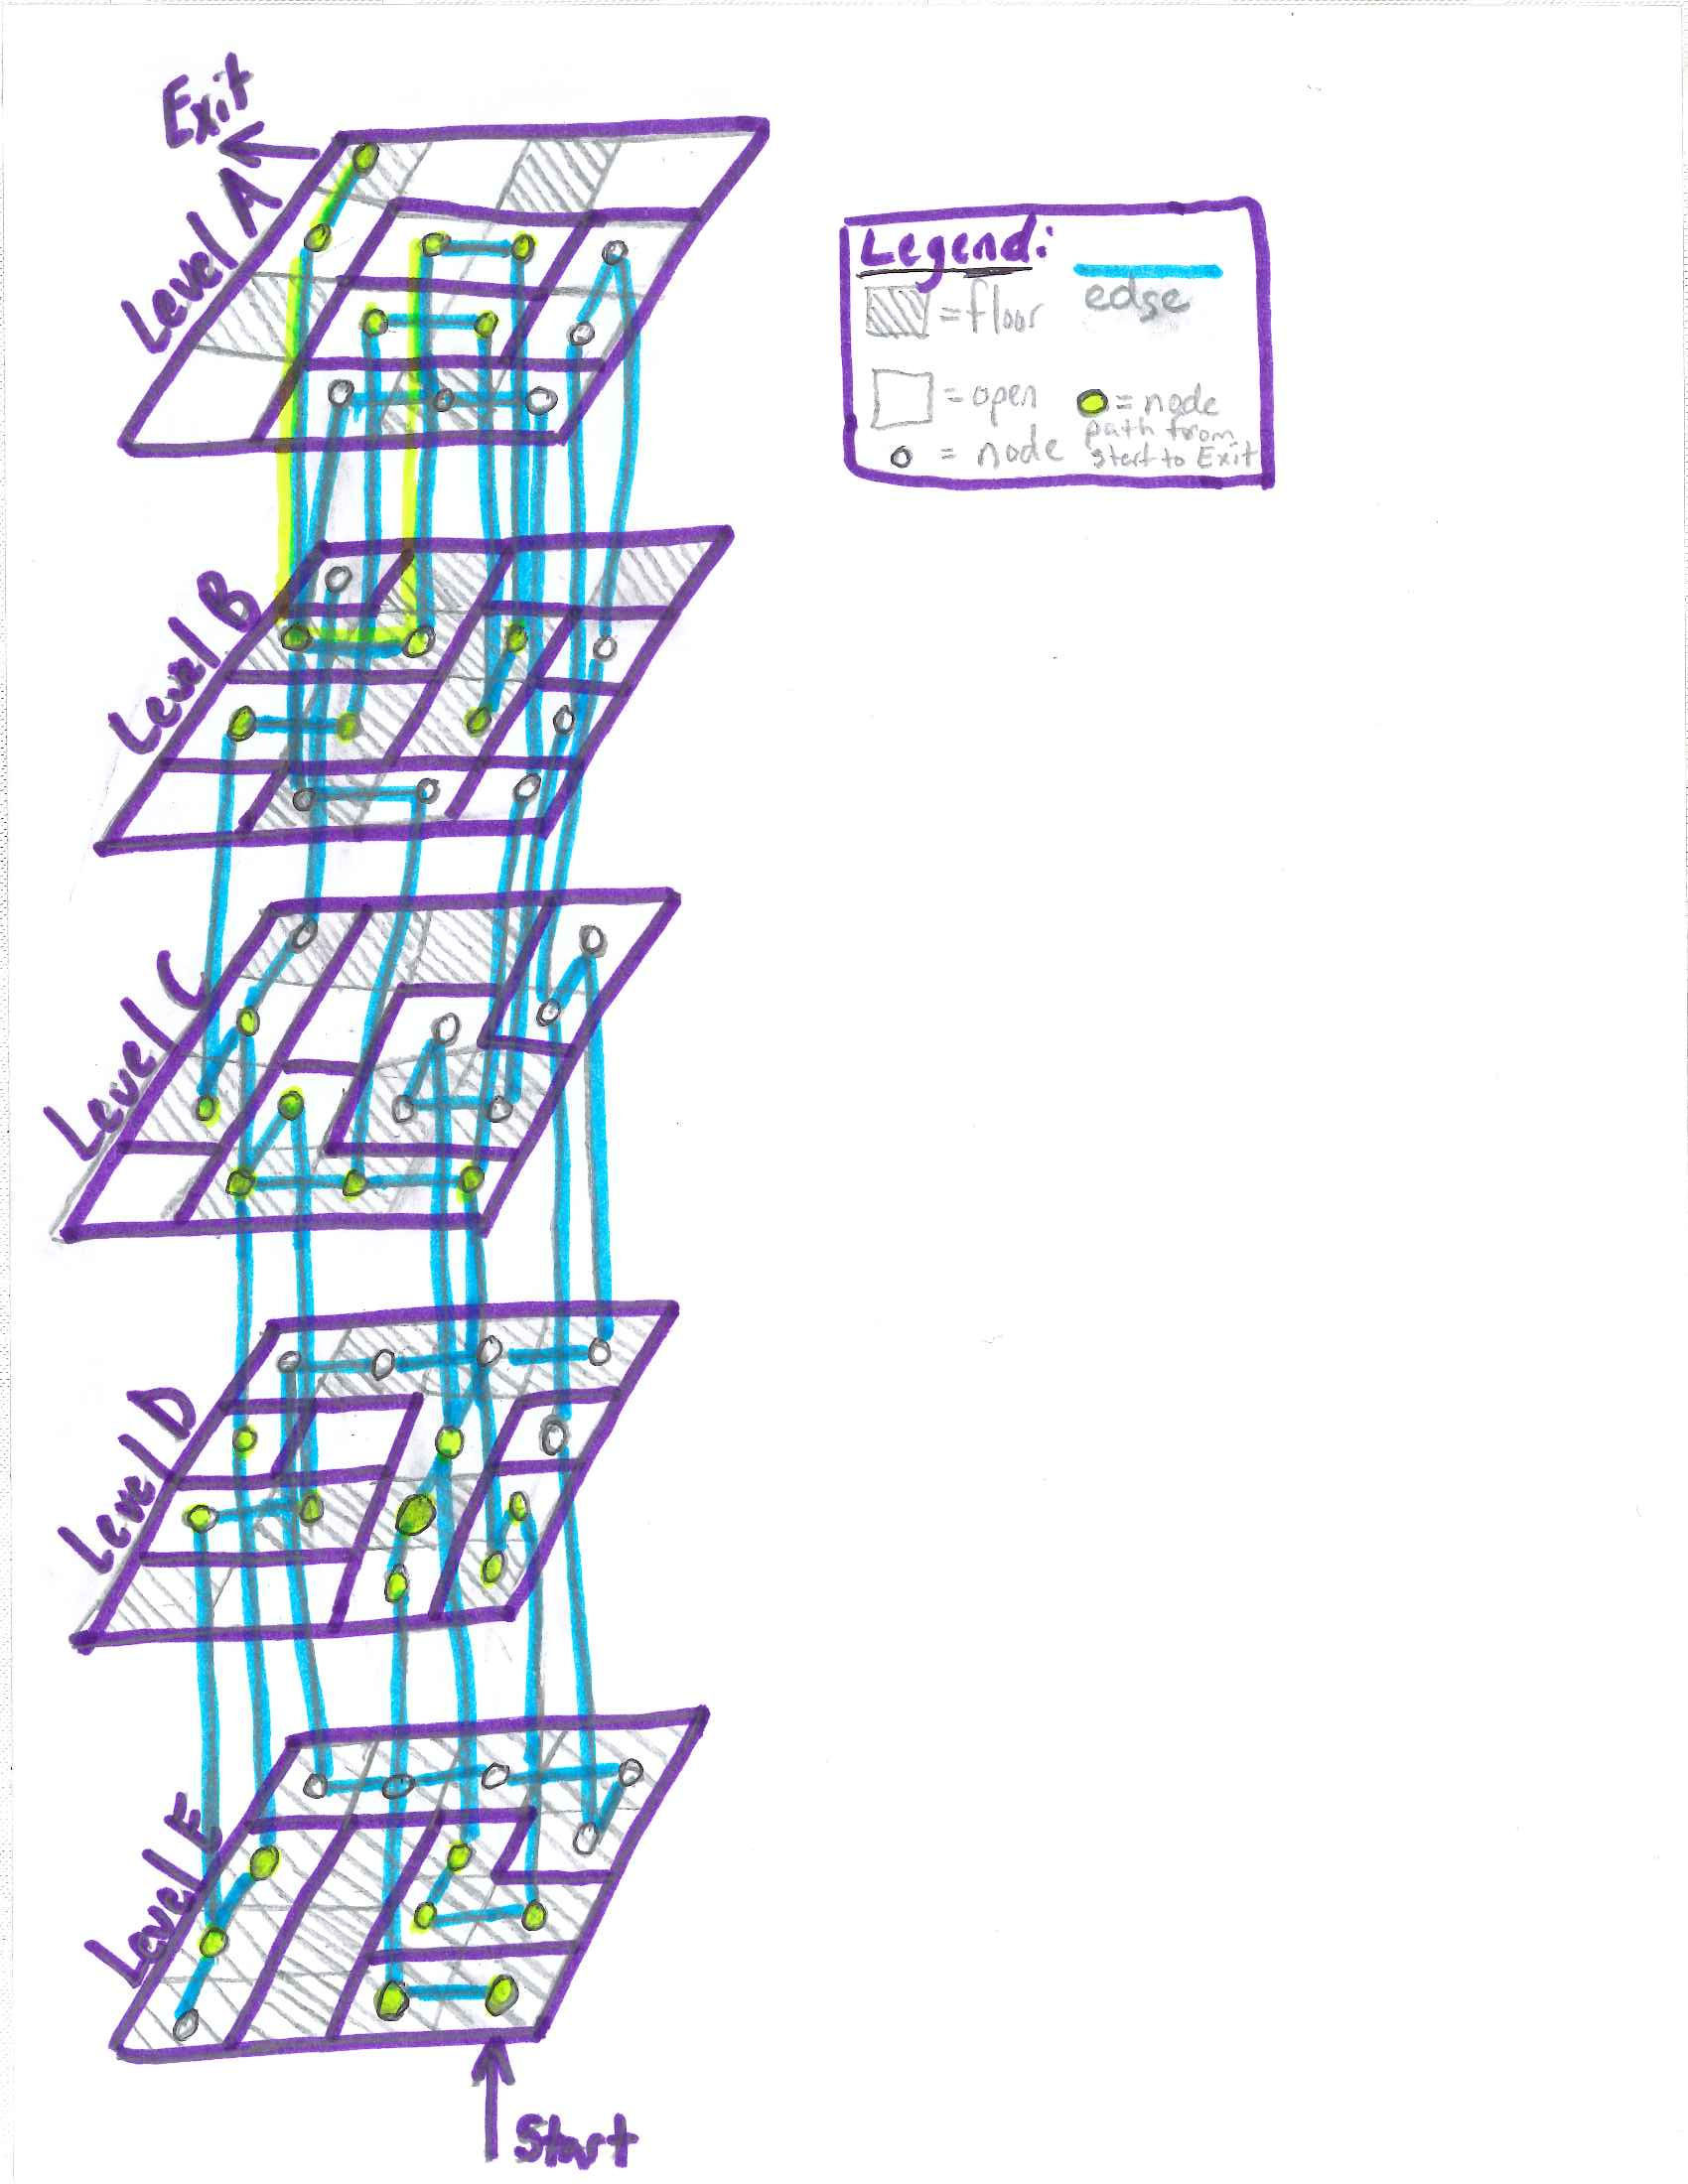
\includegraphics{figure1}

\textbf{1.3 Dijkstra's Algorithm}

Dijkstra's algorithm is the method I chose for finding any path in the three dimensional graph created. Dijkstra's algorithm is a shortest path algorithm that runs on either undirected or directed graphs to find the least cost path from initial node to a desired node. The maze problem states that we just have to find a single path from initial node to desired node in our unweighted undirected graph. I could have used the Depth-First or Breadth-first search algorithm since the three dimensional graph implemented is not weighted. However, I still chose Dijkstra's Algorithm in that case that if new inputs turned the graph into an weighted graph, the algorithm would be able to handle that change from unweighted to weighted. Also, we can apply Dijkstra's algorithm since our undirected graph is connected meaning any two nodes in the graph has an edge (which is required in Dijkstra's algorithm). We will apply the dijkstras\_path function from the NetworkX library, a Python programming library for studying complex networks, on our undirected graph to show a path from the initial node to the desired node. \\

\textbf{1.4 Prove Your Chosen Algorithm}

For the maze problem all we needed to accomplish is find a single path between the starting position and exit position. The problem can be modeled as a three dimensional graph since we can represent each square traveled to as a visited node connected by an edge to a parent node. We can use Dijkstra's algorithm so that we can examine the distance from each visited node to unvisited node until we reach our desired node (exit position). Also, Dijkstra's algorithm will be able to find the shortest path and any path from the initial node to desired node. \\

The main principle behind Dijkstra's algorithm is that if s,...,x,....,t is the shortest path between initial node to desired node, then s,...,x has to also be the shortest path between s and x. So, lets denote s as the root of the Shortest Path Tree. Next, we will denote distance traveled from s to v as d(v). Also, we will denote a set S to store each visited node in. For each node x $\epsilon$ S, d(x) is the length of the shortest s-x path. \\

Using Proof by Induction, \\

Base Case: \\
If there is only one node in set S, then set S will equal 1.

S = 1

Induction Step: \\
Let x be the current node in set S. \\

We know that for each node x that is a member of set S, d(x) is the length of the s-x path.

Let x + 1 be the next node in set S. \\

Since we know that x is a member of set S and d(x) is the length of the shortest s-x path. If node x + 1 is the next node in set S, then the distance at d(x) will denote the length of shortest s-x+1 path. This remains true since, we know that for the node x + 1 after node x is cannot be a shorter distance path from d(x).

This algorithm models which shortest path each node can take (based on the direction dictated by it's node attributes). Which will return a shortest path (a path) from the initial node to desired node.

\vspace{0.2in}
\textbf{3 Code}

\emph{Note that the information presented in this section is also included in the README file.}

For the project, we created one file: maze.py for running the maze problem program. For this program we will use console input, so in the maze.py file between lines 105 to 107, I have included a way to open and read the required input.txt file. \\

To run the maze problem program simply enter in your terminal: \\

python maze.py \\

This program will output the computed path in a file called maynes.txt. Also, the program will show a console output that should contain the same output as contained in the maynes.txt file.

\nocite{textbook, networkx, python, python-time, discrete-textbook}

\bibliography{report}{}
\bibliographystyle{plain}

\end{document}
